\documentclass[12pt]{article}

\usepackage[utf8]{inputenc}
\usepackage{graphicx}
\usepackage[spanish]{babel}

\begin{document}

\begin{titlepage}
\centering
{\bfseries\LARGE AMERIKE \par}
\vspace{1cm}
{\scshape\Large PROYECTO DE APP \par}
\vspace{3cm}
{\scshape\Huge Requerimientos funcionales y no funcionales \par}
\vspace{3cm}
\vfill
{\Large Autores: \par}
{\Large Hector Otero Caballero \par}
{\Large Jonathan Montesinos Pacheco\par}
{\Large Jose Andres Chirino \par}
{\Large Mario Perez Villalobos\par}
\vfill
{\Large Septiembre 2023 \par}
\end{titlepage}

\newpage

\section*{}

\tableofcontents

\newpage

\section{Objetivo de la aplicacion.}

\par La app que se va a realizar es un viasualizador de mangas en donde la gente podra ingresar y leer el manga que quiera.

\section{Requerimientos Funcionales.}

\begin{itemize}
	\item Visualizar mangas.
	\item Descargar archivos.
	\item Visualizar imagenes.
	\item Buscador de mangas.
	\item Visualizar sin internet.
\end{itemize}

\section{Requerimientos No Funcionales.}

\begin{itemize}
	\item Limite de descargas (5).
	\item 2 bookshelf, la privada y la de la app.
	\item Se utilizara desarollo web (laravel).
	\item visual studio 2023.
	\item Plataformas para web. 
\end{itemize}

\newpage

\section{Arquitectura.}

\begin{figure}[htbp]
	\centering
		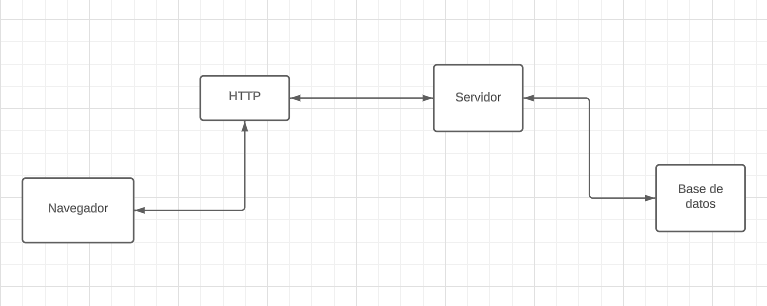
\includegraphics[width=1.00\textwidth]{Screenshot 2023-10-05 125036.png}
	\label{fig:Screenshot 2023-10-05 125036}
\end{figure}

\newpage

\section{Casos de uso.}

\begin{figure}[htbp]
	\centering
		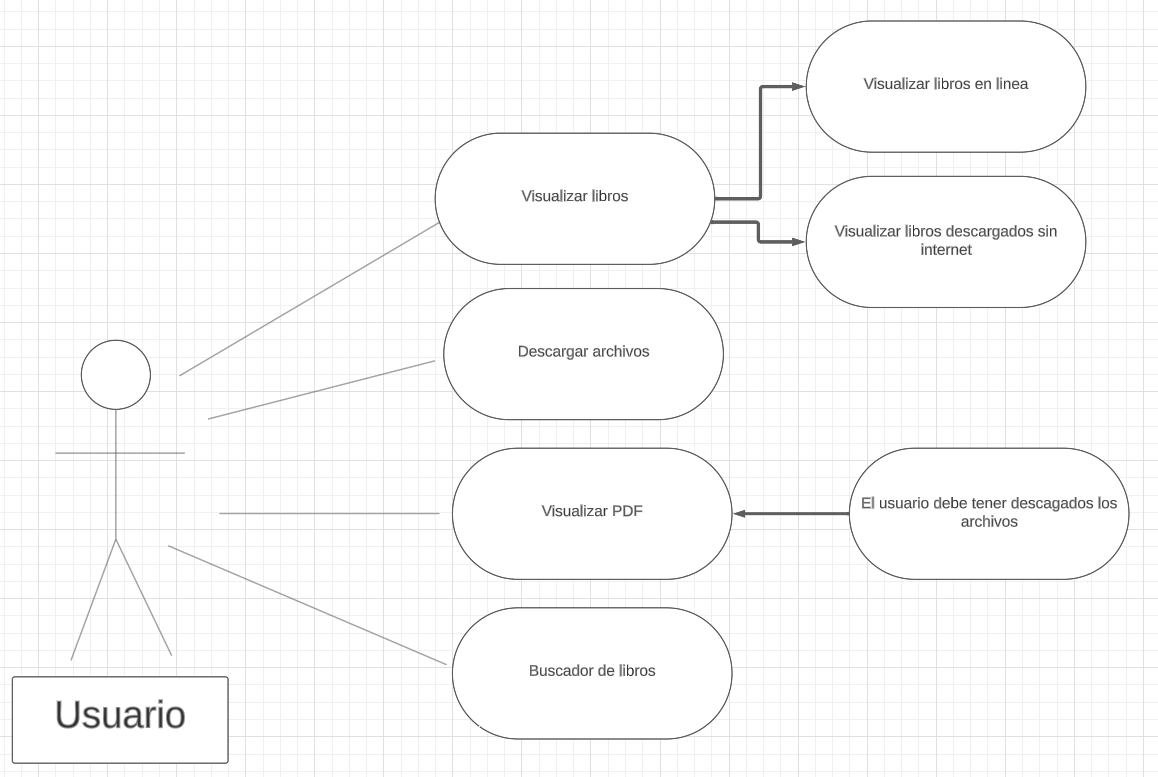
\includegraphics[width=1.00\textwidth]{Captura de pantalla 2023-09-07 124622.png}
	\label{fig:Captura de pantalla 2023-09-07 124622}
\end{figure}

\newpage

\section{Componentes.}

\begin{figure}[htbp]
	\centering
		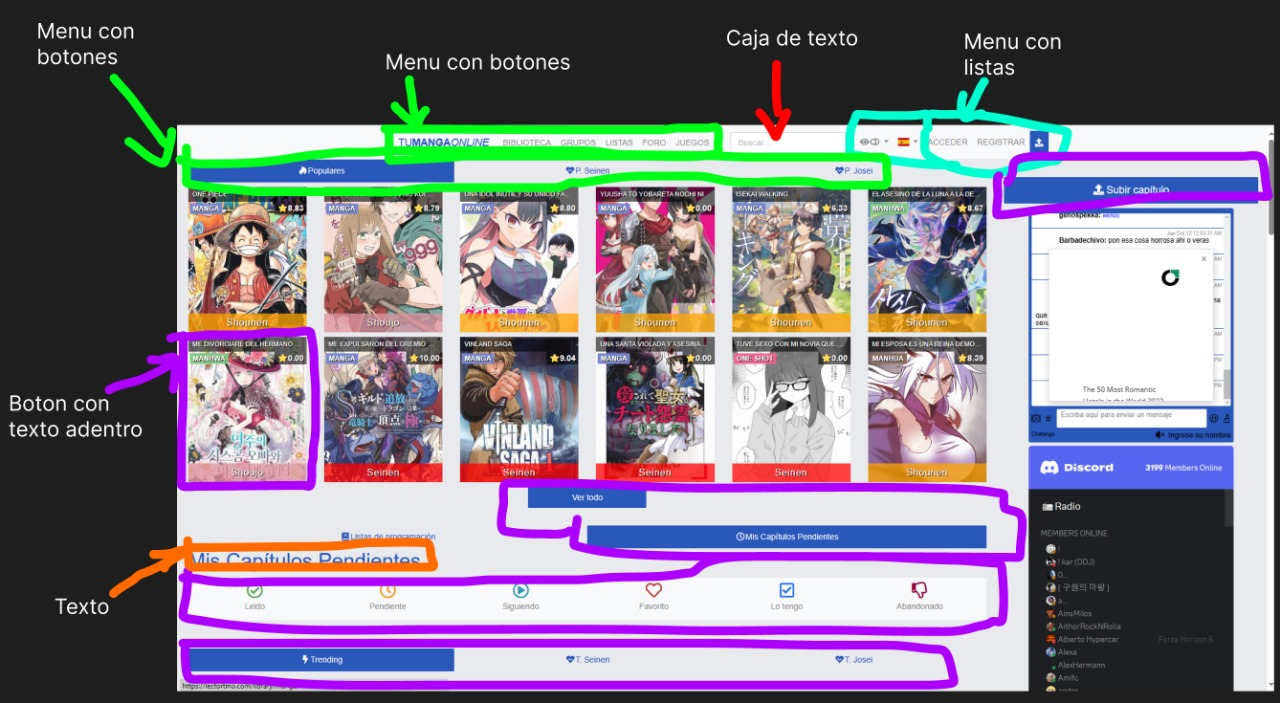
\includegraphics[width=0.85\textwidth]{Componentes.jpg}
	\label{fig:Componentes}
\end{figure}

\newpage

\section{Base de datos.}

\begin{figure}[htbp]
	\centering
		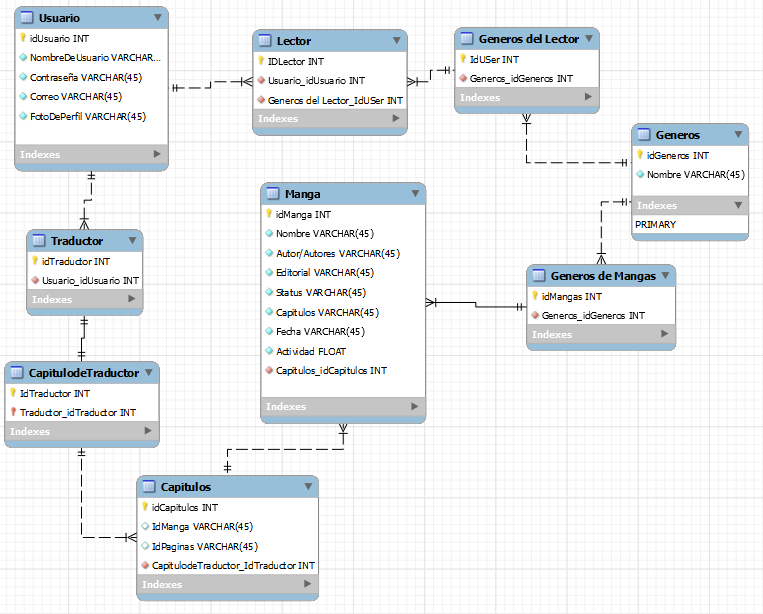
\includegraphics[width=1.00\textwidth]{Screenshot 2023-10-05 114250.png}
	\label{fig:Screenshot 2023-10-05 114250}
\end{figure}

\newpage

\section{Diagrama de clases.}

\begin{figure}[htbp]
	\centering
		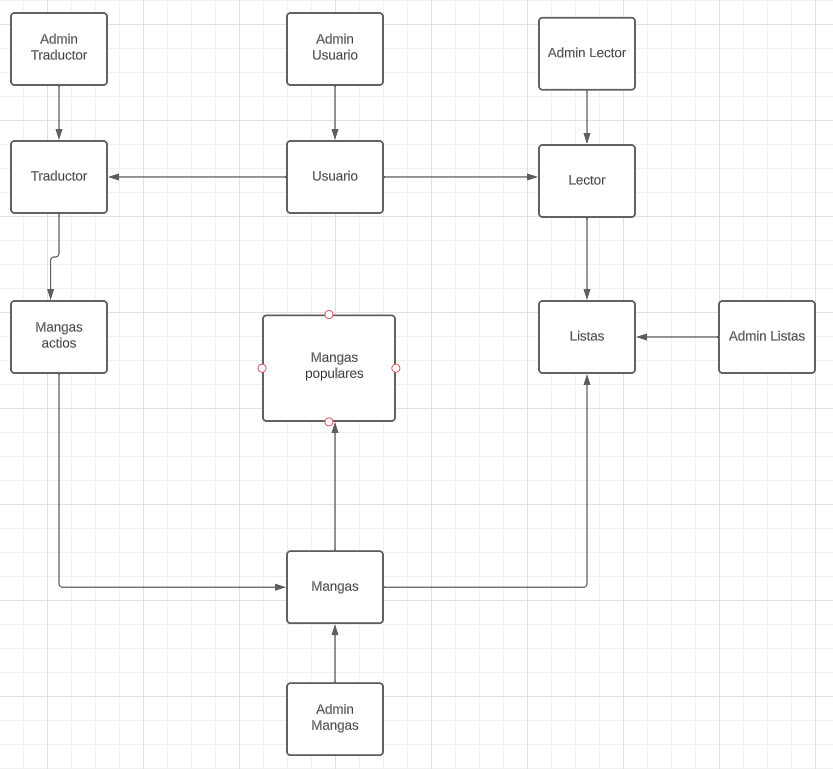
\includegraphics[width=1.00\textwidth]{Screenshot 2023-10-05 114350.png}
	\label{fig:Screenshot 2023-10-05 114350}
\end{figure}

\newpage

\section{Diagrama de secuencias.}

\begin{figure}[htbp]
	\centering
		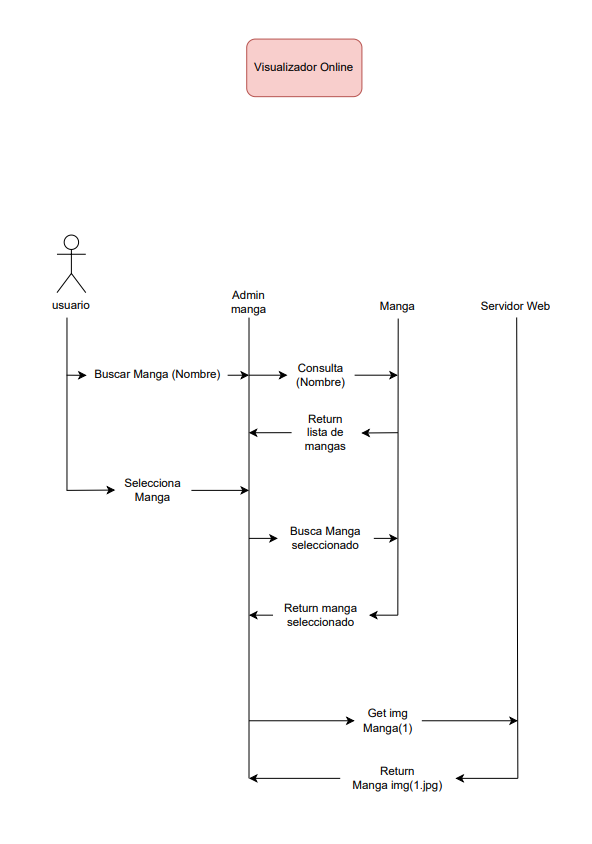
\includegraphics[width=0.75\textwidth]{Screenshot 2023-10-05 114415.png}
	\label{fig:Screenshot 2023-10-05 114415}
\end{figure}

\begin{figure}[htbp]
	\centering
		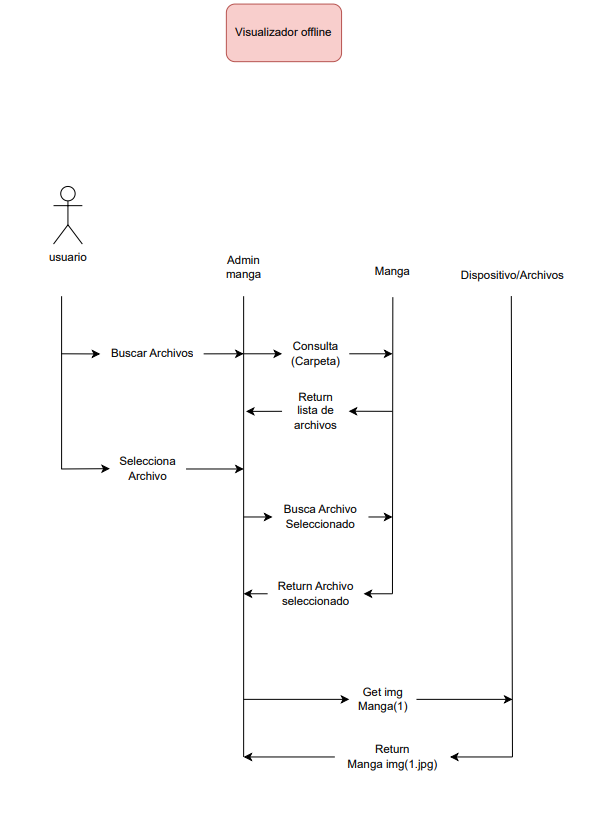
\includegraphics[width=1.00\textwidth]{Screenshot 2023-10-05 114426.png}
	\label{fig:Screenshot 2023-10-05 114426}
\end{figure}

\begin{figure}[htbp]
	\centering
		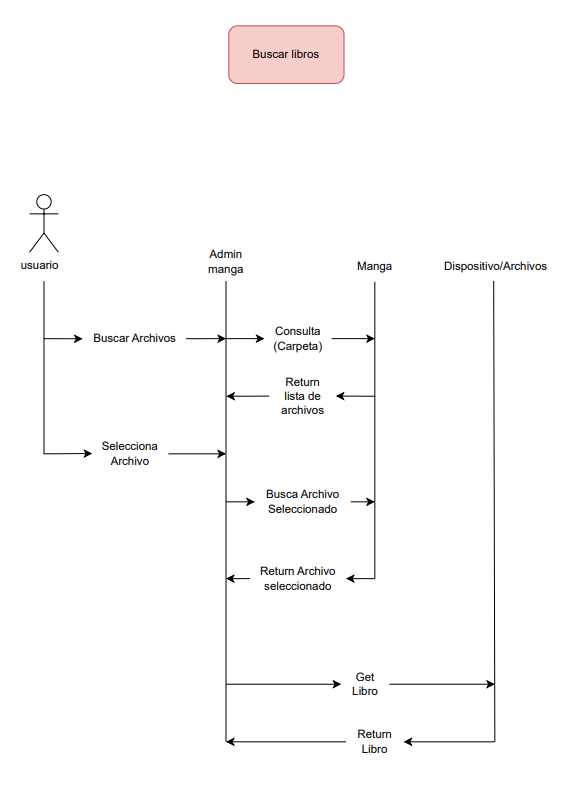
\includegraphics[width=1.00\textwidth]{Screenshot 2023-10-05 114437.png}
	\label{fig:Screenshot 2023-10-05 114437}
\end{figure}

\begin{figure}[htbp]
	\centering
		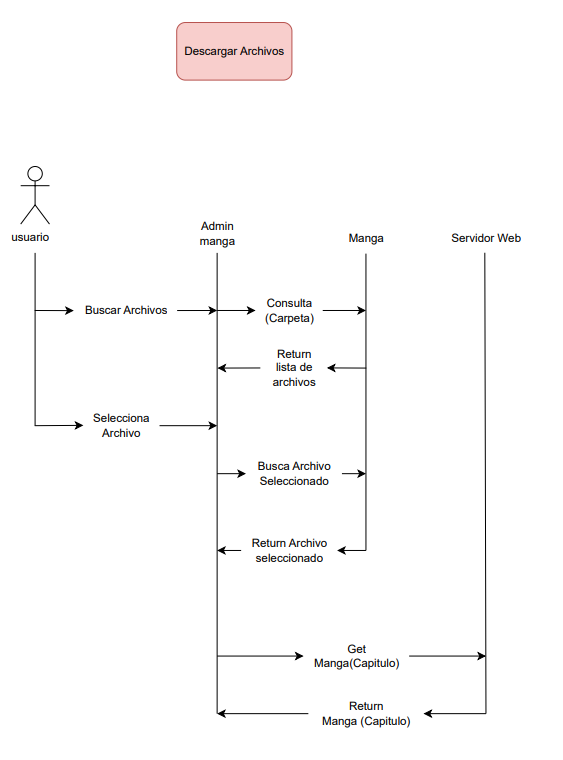
\includegraphics[width=1.00\textwidth]{Screenshot 2023-10-05 114448.png}
	\label{fig:Screenshot 2023-10-05 114448}
\end{figure}

\begin{figure}[htbp]
	\centering
		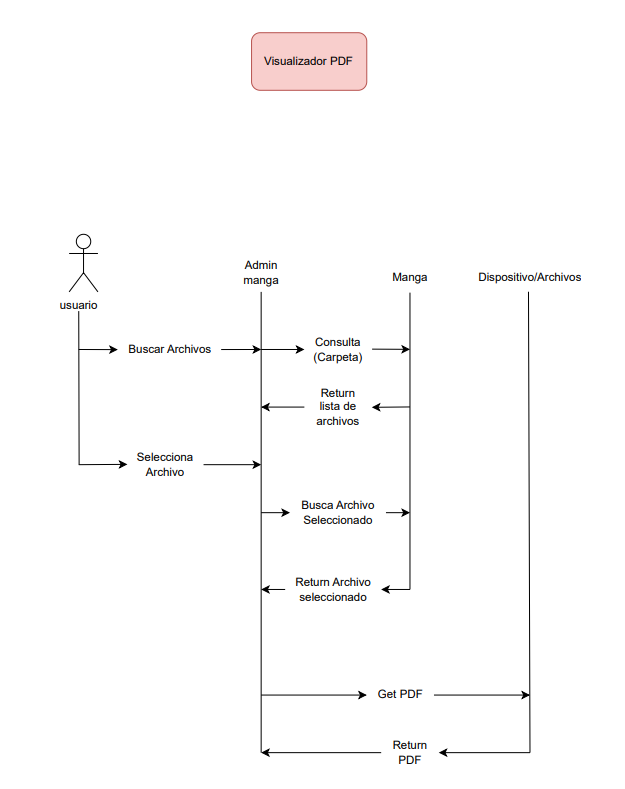
\includegraphics[width=1.00\textwidth]{Screenshot 2023-10-05 114459.png}
	\label{fig:Screenshot 2023-10-05 114459}
\end{figure}

\newpage

\section{Diagrama de flujo.}

\begin{figure}[htbp]
	\centering
		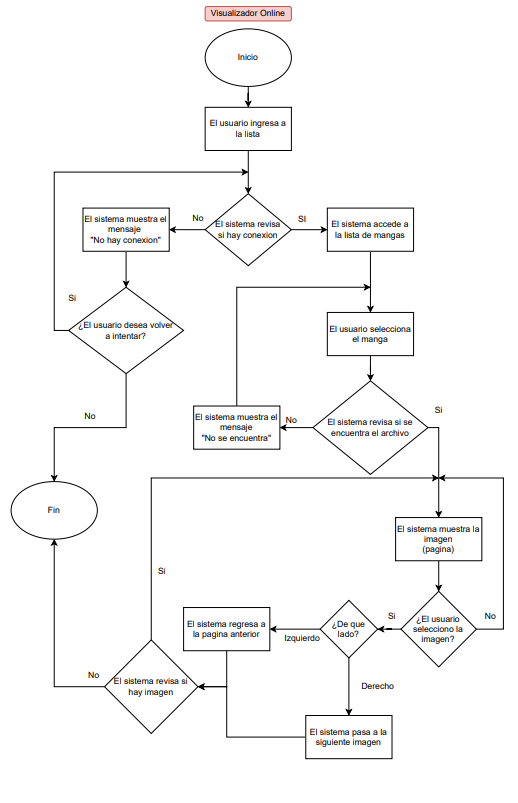
\includegraphics[width=0.70\textwidth]{Screenshot 2023-10-05 114526.png}
	\label{fig:Screenshot 2023-10-05 114526}
\end{figure}

\begin{figure}[htbp]
	\centering
		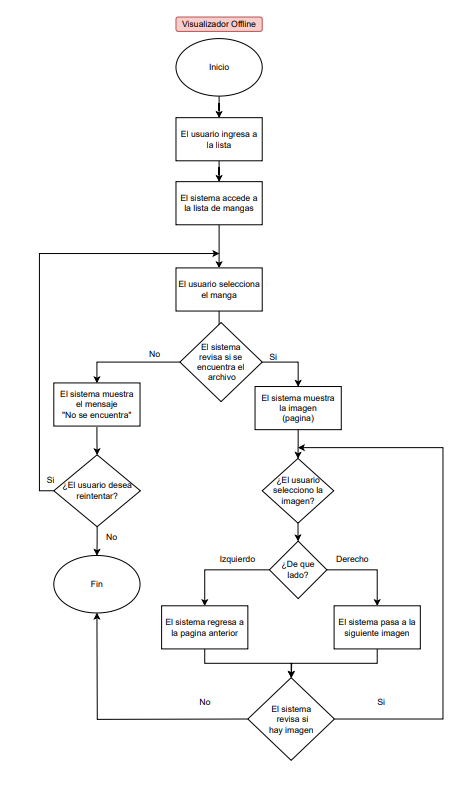
\includegraphics[width=1.00\textwidth]{Screenshot 2023-10-05 114539.png}
	\label{fig:Screenshot 2023-10-05 114539}
\end{figure}

\begin{figure}[htbp]
	\centering
		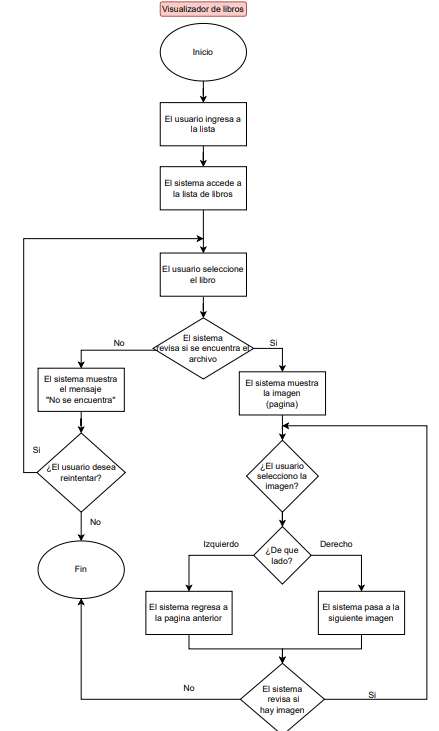
\includegraphics[width=0.75\textwidth]{Screenshot 2023-10-05 114707.png}
	\label{fig:Screenshot 2023-10-05 114707}
\end{figure}

\begin{figure}[htbp]
	\centering
		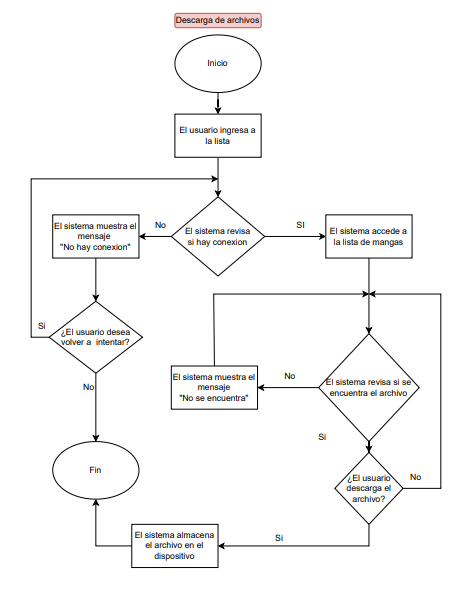
\includegraphics[width=1.00\textwidth]{Screenshot 2023-10-05 114715.png}
	\label{fig:Screenshot 2023-10-05 114715}
\end{figure}

\begin{figure}[htbp]
	\centering
		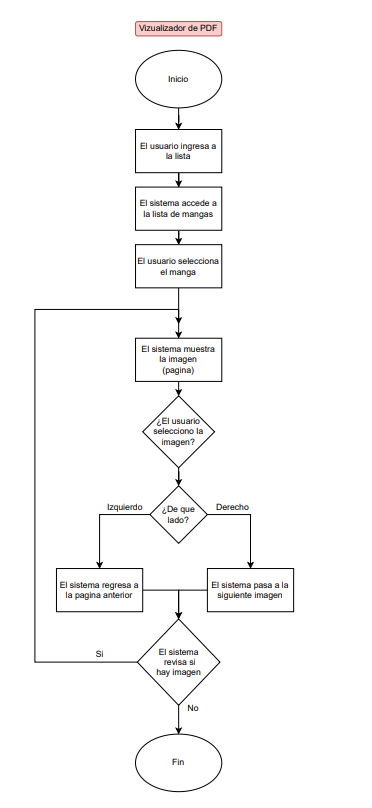
\includegraphics[width=0.75\textwidth]{Screenshot 2023-10-05 114725.png}
	\label{fig:Screenshot 2023-10-05 114725}
\end{figure}

\newpage

\section{Diagrama de estado.}

\begin{figure}[htbp]
	\centering
		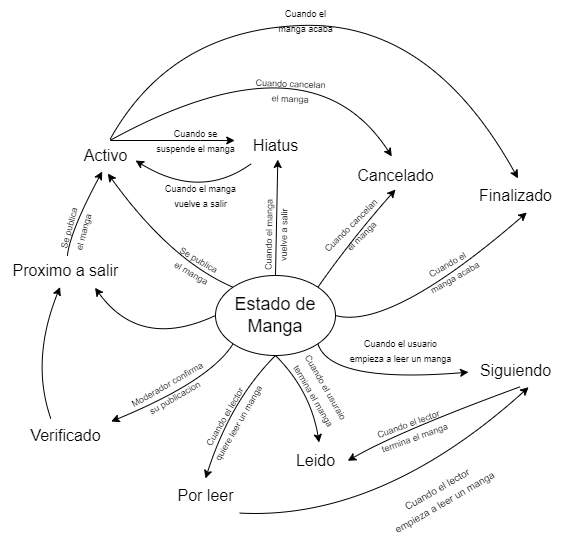
\includegraphics[width=0.85\textwidth]{Diagrama_estado.png}
	\label{fig:Diagrama_estado}
\end{figure}

\newpage

\section{Mapa de sitio.}

\begin{figure}[htbp]
	\centering
		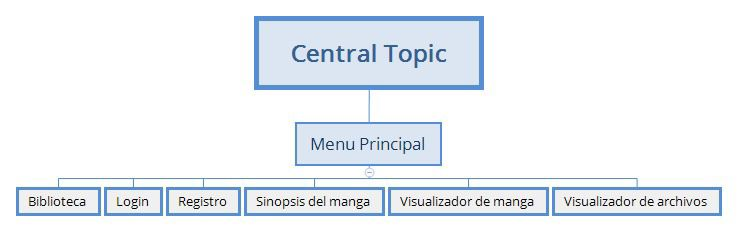
\includegraphics[width=0.85\textwidth]{mapa_sitio.jpg}
	\label{fig:mapa_sitio}
\end{figure}

\newpage

\section{Identidad.}

\begin{figure}[htbp]
	\centering
		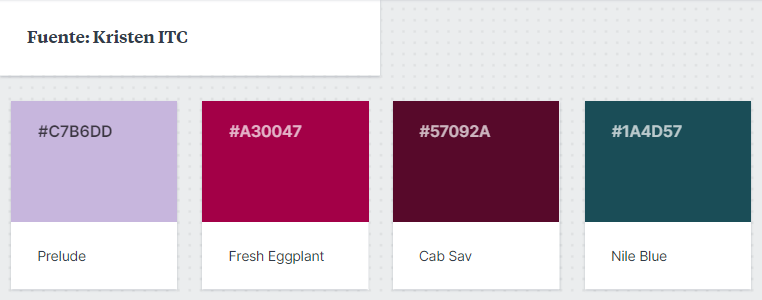
\includegraphics[width=0.85\textwidth]{fuente_colores.png}
	\label{fig:fuente_colores}
\end{figure}

\begin{figure}[htbp]
	\centering
		
\includegraphics[width=0.90\textwidth]{logo.jpg}
	\label{fig:logo}
\end{figure}

\newpage

\section{Prototipo en figma.}

\par link a figma \url{https://www.figma.com/file/yCJqW1hXGkLWojVEB5c7S9/Untitled?type=design&node-id=0-1&mode=design&t=4i90prLvQj9c54Nh-0}

\begin{figure}[htbp]
	\centering
		
\includegraphics[width=0.85\textwidth]{Desktop - 1.png}
	\label{fig:Desktop - 1}
\end{figure}

\newsection
\end{document}